\documentclass{winnower}
\usepackage{indentfirst}
\usepackage{graphicx}
\usepackage{caption}
\usepackage{subfigure}
\usepackage{xcolor}
\usepackage{float}
\usepackage[section]{placeins}
\usepackage{multirow}
\usepackage{booktabs}
\setlength{\belowcaptionskip}{-0.5cm}

\begin{document}

\title{Homework6 report}

\author{Haoyu Guan}

\affil[1]{Questrom School of Business, Boston University}







\date{2020.02.11}

\maketitle




%-------------------------------------------------%
\section{Numerical PDEs:}
%-------------------------------------------------%


\indent Suppose that the underlying security SPY evolves according to standard geometric brownian motion. Then its derivatives obey the Black-Scholes equation:

%\vspace{12 pt}
$$
\frac{\partial c}{\partial t}+\frac{1}{2} \sigma^{2} s^{2} \frac{\partial^{2} c}{\partial s^{2}}+r s \frac{\partial c}{\partial s}-r c=0
$$


Use SPY's closing price on March $4,2020$.


We are going to find the price of a call spread with the right of early exercise. The two strikes of the call spread are $K_{1}=315$ and $K_{2}=320$ and the expiry is September $30,2020$
\\





\textbf{1. Explain why this instrument is not the same as being long an American call with strike 315 and short an American call with strike 320 , both with expiry September $30,2020$.}
\\

It is a totally different thing. Because short an American option that means you do not have the right of early exercise but your opponent does. So that is different from a call spread with the right of early exercise.
\\

\textbf{2. For riskless rate $r,$ use the 3-month US Treasury bill at the close of March 4, 2020. Say where you got the rate and why you consider it a reliable source.}
\\

$r=0.72\%$ which is from the government website.
\\



\textbf{3. Let's assume that we are not able to find $\sigma$ by calibrating to the European call spread price and must find it by other means. Find a way to pick the $\sigma,$ explain why you chose this method, and then find the $\sigma$.}
\\

So we apply linear interpolation to acquire the implied volatility of 315 and 320. And then take the average of this 2 volatility. so the $\sigma$ is 0.2183167.
\\

\textbf{4. Set up an explicit Euler discretization of (1). You will need to make decisions about the choice of $s_{\max }, h_{s}, h_{t},$ etc. Please explain how you arrived at each of these choices.}
\\

As we all know the $S_0$ is near the $320$. So I would choose $S_{max}=600$ which would be big enough to calculate the price. And $T=\frac{7}{12}$. So I built a $M\times N$ scheme where $M=300,N=3000$. By that way, we can get $h_s=\frac{S_{max}}{M}=1$ and $h_t=\frac{T}{N}=\dfrac{\frac{7}{12}}{3000}$


\newpage
\textbf{5. Let $A$ be the update matrix that you created in the previous step. Find out its eigenvalues and check their absolute values.}
\\


\begin{figure*}[!h]
\begin{center}
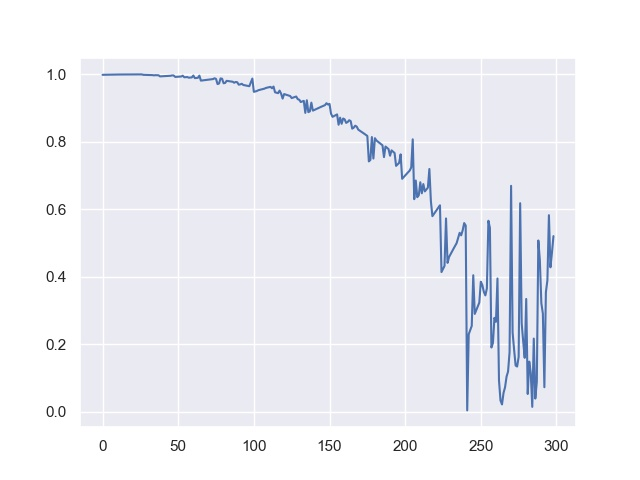
\includegraphics[scale=0.7]{1_1.jpg}
\caption
{eiegnvalue of A}
\label{fig:f1}
\end{center}
\end{figure*}

\begin{figure*}[!h]
\begin{center}
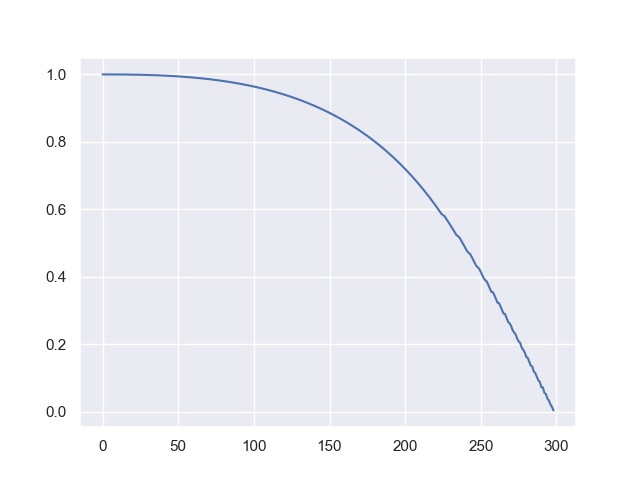
\includegraphics[scale=0.7]{1_2.jpg}
\caption
{ordered eigenvalue of A}
\label{fig:f1}
\end{center}
\end{figure*}


\textbf{6. Apply your discretization scheme to find today's price of the call spread without the right of early exercise. The scheme will produce a whole vector of prices at time $0 .$ Explain how you chose the one for today's price.}
\\

I get $C_0=2.1996583210559235$ by using

$$\left[\begin{array}{ccccc}
a_{1} & u_{1} & & & \\
l_{2} & a_{2} & u_{2} & & \\
& \ddots & \ddots & \ddots & \\
& & l_{M-2} & a_{M-2} & u_{M-2} \\
& & & l_{M-1} & a_{M-1}
\end{array}\right]\left[\begin{array}{c}
C\left(s_{1}, t_{j}\right) \\
C\left(s_{2}, t_{j}\right) \\
\vdots \\
C\left(s_{M-2}, t_{j}\right) \\
C\left(s_{M-1}, t_{j}\right)
\end{array}\right]+\left[\begin{array}{c}
0 \\
0 \\
\vdots \\
0 \\
b_{j}
\end{array}\right]$$

where
$$b_{j}=u_{M-1}\left(s_{M}-K e^{-r\left(t_{N}-t_{j}\right)}\right)$$
\\

\textbf{7. Modify your code in the previous step to calculate the price of the call spread with the right of early exercise. What is the price?}
\\

I get $C_0=4.424891870026654$ and the eigenvalue

\begin{figure*}[!h]
\begin{center}
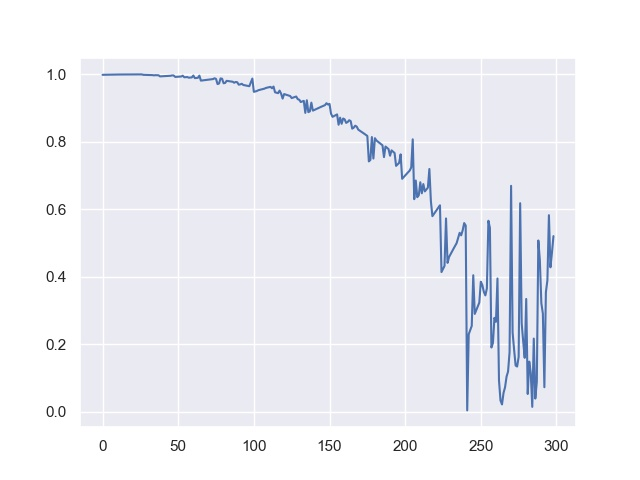
\includegraphics[scale=0.7]{1_3.jpg}
\caption
{eigenvalue of A}
\label{fig:f1}
\end{center}
\end{figure*}

\begin{figure*}[!h]
\begin{center}
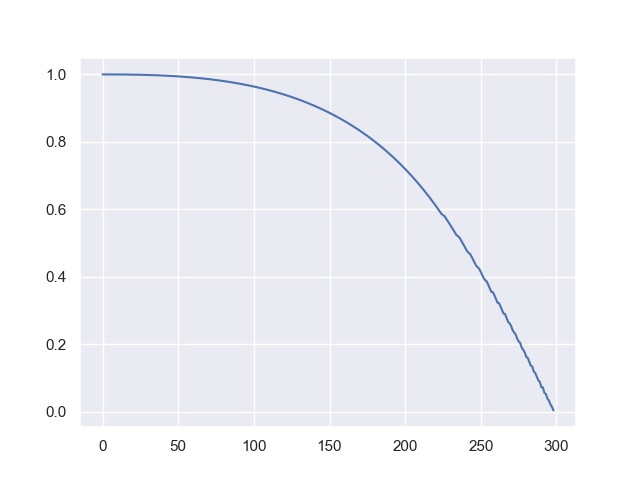
\includegraphics[scale=0.7]{1_4.jpg}
\caption
{ordered eigenvalue of A}
\label{fig:f1}
\end{center}
\end{figure*}


\newpage
\textbf{8. Calculate the early exercise premium as the difference between the American and European call spreads. Is it reasonable?}
\\

I get $premium=2.2252335489707304$ which is reasonable because price of early premium is larger than price without it.










\end{document}
